\documentclass[a4paper,11pt]{scrartcl}
\usepackage[T1]{fontenc}
\usepackage[utf8]{inputenc}
\usepackage{lmodern}
\usepackage[spanish]{babel}
\usepackage{mathtools}
\usepackage{amssymb, amsmath, amsbsy}
\usepackage{float}
\usepackage{enumerate}
\usepackage{graphicx}
\usepackage{subfigure}
\usepackage{hyperref}

\title{Trabajo y energía e impulso y cantidad de movimiento de la partícula}
\subtitle{Tercer Examen Parcial \\ Equipo 12}
\author{
  Aguilar Enriquez Paul Sebastian\\
  \and
  Benitez Barroso Brandon Raul\\
  \and
  Castillo Herrera Gabriela\\
  \and
  Martinez Vidal Joceline Yadira\\
  \and
  Milán Hernández Maria Fernanda
  }
\date{10 de octubre del 2016}
\begin{document}

\maketitle

\begin{center}
  Repositorio del documento en GitHub
  \url{https://github.com/penserbjorne/clase-cinematicaydinamica-2017-1}
\end{center}

\textbf{Ejercicio 28} En clase vimos que el potencial gravitacional está dado por\\
\begin{center}
  $V(r) = -G \frac{M_T m}{r}$
\end{center}

donde $M_T$ es la masa de la Tierra, $m$ es la masa de la partícula bajo estudio, y $r$ es la distancia entre el centro de la Tierra y la partícula. Calcula, usando sólo la conservación de energía, la \textit{velocidad de escape} que debe imprimirse a la partícula para que ésta no caiga de nuevo a la tierra. Evalúa tu resultado si $G \simeq 6.67 \times 10^{-11} [\frac{m^3}{kg*s^2}], M_T \simeq 6 \times 10^24 kg$ y el radio de la Tierra es $R \simeq 6.371 km$.\\

\textbf{Solución:}

\begin{center}

$E_{mc} = V + E_c = 0$\\
\hfill \break
$-G\frac{M_T m}{r} + \frac{1}{2} m v^2 = $\\
\hfill \break
$6 371 km = 6 371 000 m$\\
\hfill \break
$\frac{1}{2} m v^2 = G\frac{M_T m}{r}$\\
\hfill \break
$\frac{1}{2} v^2 = G\frac{M_T}{r}$\\
\hfill \break
Velocidad de escape : $V = \sqrt{\frac{2 G M_T}{r}}$\\
\hfill \break
$V = \sqrt{\frac{2 * 6.67\times10^{-11}[\frac{m^3}{kg*s^2}]}{6 371 000 [m]} 6\times10^{24}[kg]}$\\
\hfill \break
$V = \sqrt{\frac{2 * 6.67\times10^{-11}}{6 371 000} 6\times10^{24}[kg] \frac{m^2}{s^2}}$\\
\hfill \break

\begin{equation}
  \left\lbrace
  \begin{array}{l}
    V = 11208.5578 \frac{m}{s} = 11.2086 \frac{km}{s}
  \end{array}
  \right.
\end{equation}

 
\end{center}

\textbf{Ejercicio 33} Una de las codiciones para que una pelota de tenis sea utilizada en una competecia oficial es que, al dejarla caer desde una altura de 1${\bf [m]}$, ésta rebota entre 50 y 60${\bf [cm]}$. Determina el rango de coeficientes de restitución que puede tener la pelota para que esto suceda. \\

\textbf{Solución:}

\begin{figure}[H]
  \centering
  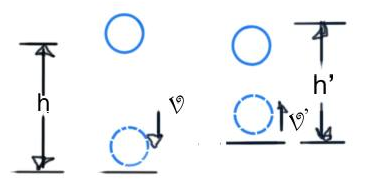
\includegraphics[height=4cm]{33_1}
  \caption{Energias potenciales.}
  \label{fig:33_1}
\end{figure}

\begin{center}

Con el movimiento uniformemente acelerado, tenemos que: \\
\begin{center}
$v =   \sqrt{2gh}  $ \\
\begin{equation}
v' =    \sqrt{2gh'}
\end{equation}
\end{center}

Por coeficiente de restitución: \\
\begin{center}
$e =  \dfrac{v'}{v}     $ \\
\begin{equation}
v' =    \sqrt{\dfrac{h'}{h}}
\end{equation}
\end{center}

Sabiendo que la altura de la caída es de 1[m].\\
Y el rango de la altura de rebote es de: $ 0.5 \leq h' \leq 0.6$\\

Entonces, tenemos: \\
\begin{center}
$  \sqrt{\dfrac{0.5}{1}} \leq e \leq  \sqrt{\dfrac{0.6}{1}}$\\
\end{center}
\begin{center}
$\dfrac{ \sqrt{2}}{2} \leq e \leq \dfrac{ \sqrt{15}}{5}$\\
\end{center}
\begin{center}
$0.70710 \leq e \leq 0.7745$\\
\end{center}

Por lo tanto el rango de coeficiente de restitución es:
\begin{equation*}
  \left\lbrace
  \begin{array}{l}
    0.70710 \leq e \leq 0.7745
  \end{array}
  \right.
\end{equation*}


\end{center}

\textbf{Ejercicio 35} Dos objetos se deslizan sobre una superficie horizontal sin fricción. El primer objeto, con
masa $m_1 = 5 [kg]$ se mueve con una velocidad $v_1 = 4.5 [\frac{m}{s}]$ hacia el segundo objeto, con masa $m_2 =  2.5 [kg]$, el  cual  está  inicialmente  en reposo.  Después  de  la  colisión, ambos
objetos se mueven con velocidades que hacen un ángulo de $30^{\circ}$ en cada lado de la línea de movimiento original del primer objeto.(a) ¿Cuáles son las velocidades de ambos objetos después de la colisión? (b) ¿la colision es elástica o inelástica?\\

\textbf{Solución:}

\begin{center}
a)\\
\hfill \break

\begin{figure}[H]
  \centering
  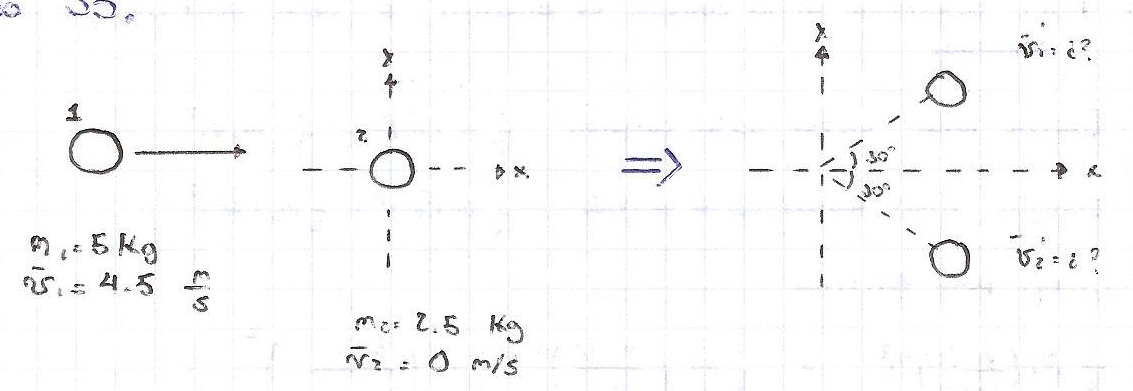
\includegraphics[height=5.5cm]{35_1}
  \caption{Diagrama de cuerpo libre.}
  \label{fig:35_1}
\end{figure}

Cantidad de movimiento de un objeto $\bar{p} = m \bar{v}$\\
\hfill \break
Sistema de ecuaciones:\\
\begin{equation}
  m_1 v_1 = m_1 {v_1}' cos(\theta) + m_2 {v_2}' cos(\theta)
\end{equation}

\begin{equation}
  m_1 {v_1}' sen(\theta) = m_2 {v_2}' sen(\theta) \Rightarrow m_1 {v_1}' = m_2 {v_2}'  
\end{equation}

De (5)\\
\hfill \break
\begin{equation}
  {v_1}' = \frac{m_2 {v_2}'}{m_1}
\end{equation}

Sustituyendo (6) en (4)\\
\hfill \break
$m_1 v_1 = m_1(\frac{m_2 {v_2}'}{m_1} cos(\theta) + m_2 {v_2}' cos(\theta)$\\
\hfill \break
$m_1 v_1 = 2 m_2 {v_2}' cos(\theta)$\\
\hfill \break
$2 m_2 {v_2}' = \frac{m_1 v_1}{cos(\theta)}$\\
\hfill \break
\begin{equation}
{v_2}' = \frac{m_1 v_1}{2 m_2 cos(\theta)}
\end{equation}

Sustituyendo valores en (7)\\
\hfill \break
\begin{equation*}
  \left\lbrace
  \begin{array}{l}
    {v_2}' = \frac{5 * 4.5}{2 * 2.5 * cos(30^\circ)} \frac{kg * \frac{m}{s}}{kg} = 3\sqrt{3} [\frac{m}{s}] = 5.196 [\frac{m}{s}]
  \end{array}
  \right.
\end{equation*}

Sustituyendo valores en (3)\\
\hfill \break
\begin{equation*}
  \left\lbrace
  \begin{array}{l}
    {v_1}' = \frac{2.5 * 3\sqrt{3}}{5} \frac{kg * \frac{m}{s}}{kg} = \frac{3\sqrt{3}}{2} [\frac{m}{s}] = 2.598 [\frac{m}{s}]
  \end{array}
  \right.
\end{equation*}

b) Para determinar si la colision es elastica, se debe verificar que la energia se conserve.\\
\hfill \break
Energia total antes de la colision: $\frac{1}{2} m_1 \bar{v_1}^2 = \frac{1}{2} m_1 {v_2}^2$\\
\hfill \break
Energia total antes de la colision: $\frac{1}{2} m_1 \bar{v_1}'^2 = \frac{1}{2} m_1 {v_2}'^2$\\
\hfill \break
Igualamos para verificar\\
\hfill \break
$\frac{1}{2} m_1 {v_1}^2 = \frac{1}{2} m_1 {v_1}'^2 + \frac{1}{2} m_2 {v_2}'^2$\\
\hfill \break
$\frac{1}{2} m_1 {v_1}^2 = \frac{1}{2} (m_1 {v_1}'^2 + m_2 {v_2}'^2)$\\
\hfill \break
$m_1 {v_1}^2 = m_1 {v_1}'^2 + m_2 {v_2}'^2$\\
\hfill \break
$5 * {4.5}^2 = 5 {\frac{3\sqrt{3}}{2}}^2 + 2.5 {3\sqrt{3}}^2$\\
\hfill \break
$101.25 = 33.75 + 76.5$\\

\begin{equation*}
  \left\lbrace
  \begin{array}{l}
    101.25 = 101.25
  \end{array}
  \right.
\end{equation*}
\end{center}

\textbf{Ejercicio Extra} A la bola de la figura~\ref{fig:Extra_1}, de masa de $m$ =  1[kg] que cuelga en el punto ${\bf A}$ por una cuerda inextensible de longitud  \emph{l} se le imprime una velocidad $v_{0} = 5 [m/s]$. Si  \emph{l}= 1[m]  $x_{B} = 10 [cm]$, determina $y_{B}$ de tal manera que la bola entre en la canasta.\\

\begin{figure}[H]
  \centering
  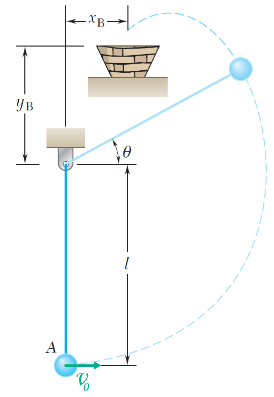
\includegraphics[height=7cm]{Extra_1}
  \caption{Sistema mostrado para el problema extra.}
  \label{fig:Extra_1}
\end{figure}

\textbf{Solución:}

\begin{center}

Posicionandonos en A, tenemos que: \\
\begin{center}
$v_{1} = v_{0}  $ \\
\end{center}

Poniendo en una posición 2 sea el punto descrito por el ángulo en que la trayectoria de la pelota cambia de circular a parabolico. En la posición 2, la tensión Q en el cable es cero.\\
Relacionando $v_{2}$ y $\theta$ basado e Q=0, tenemos el diagrama de cuerpo libre, que es:\\

\begin{figure}[H]
  \centering
  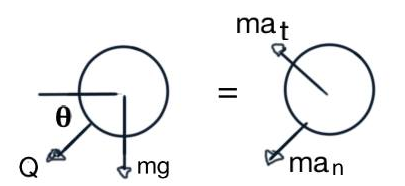
\includegraphics[height=4cm]{Extra_2}
  \caption{Diagramas de cuerpo libre.}
  \label{fig:Extra_2}
\end{figure}

\begin{center}
\[
\sum F= 0: Q + mg \sen(\theta) = ma_{n} = \dfrac{m{v_{2}}^{2}}{\emph{l}}
\] \\
\end{center}

Con:\\
\begin{equation}
 Q = 0, m{v_{2}}^{2} = g\emph{l}\sen(\theta)  o con v_{2} = \sqrt{g\emph{l}\sen(\theta)}
\end{equation}

Relacionando $v_{0}$ entre $v_{2}$ y $\theta$ basado en la conservación de la energía. \\

\begin{center}
$T_{1} + V_{1} = T_{2} + V_{2}$\\
\end{center}
\begin{center}
$\dfrac{1}{2}m{v_{0}}^{2} - mg\emph{l} = \dfrac{1}{2}m{v_{2}}^{2} + mg\emph{l}\sen(\theta) $\\
\end{center}
\begin{center}
\begin{equation}
{v_{0}}^{2} - {v_{2}}^{2} = 2g\emph{l}(1 + \sen(\theta))
\end{equation}
\end{center}

Eliminando $v_{2}$ de la equación (1) y (2), tenemos:\\
\begin{center}
${v_{0}}^{2} - g\emph{l}\sen(\theta) = 2g\emph{l}(1 + \sen(\theta))$\\
\end{center}
\begin{center}
$\sen(\theta) = \dfrac{1}{3}\left[\dfrac{{v_{0}}^{2}}{g\emph{l}} - 2\right] =  \dfrac{1}{3}\left[\dfrac{5^{2}}{(9.81)(1)} - 2\right] = 0.849473 $\\
\end{center}
\begin{center}
$\theta = 58.154^{\circ} $
\end{center}

De la equación (1), tenemos que:\\
\begin{center}
${v_{2}}^{2} = (9.81)(1)\sen(58.154^{\circ}) = 8.33329 m^{2}/s^{2} $\\
\end{center}
\begin{center}
$v_{2} = 2.88674 m/s$\\
\end{center}

Teniendo como "x" y "y" coordenadas en la posición 2:\\
\begin{center}
$x_{2} = \emph{l}\cos(\theta) = (1)\cos(58.154^{\circ}) = 0.52763 m $\\
\end{center}
\begin{center}
$y_{2} = \emph{l}\sen(\theta) = (1)\sen(58.154^{\circ}) = 0.849469 $\\
\end{center}

$t_{2}$ es el tiempo cuando la pelota esta en la posicion 2.\\
Teniendo el movimiento en la trayectoria parabólica. El movimiento horizontal es:\\
\begin{center}
$\dot{x}_{2} = -v_{2}\sen(\theta) = -2.88674\sen(58.154^{\circ}) = -2.45219^{\circ} $\\
\end{center}
\begin{center}
$x = x_{2} - 2.45219(t - t_{2})$\\
\end{center}

En el punto B, tenemos:\\
\begin{center}
$x_{B} = 0.1 m $\\
\end{center}
\begin{center}
0.1 = $ 0.52763 - 2.45219(t_{B} - t_{2})$\\
\end{center}

Por lo que:\\
\begin{center}
$t_{B} - t_{2} = 0.174386$\\
\end{center}

El movimiento vertical en el punto B es:\\
\begin{center}
$y_{B} = y_{2} + v_{2}\cos(\theta)(t_{B} - t_{2}) - \dfrac{1}{2}g(t_{B} - t_{2})^{2}$\\
\end{center}
\begin{center}
$y_{B} = 0.849469 + (2.88674\cos(58.154^{\circ}))(0.174386) - \dfrac{1}{2}(9.81)(0.174386)^{2} = 0.9659222 $\\
\end{center}

Por lo tanto $y_{B}$ es:
\begin{equation*}
  \left\lbrace
  \begin{array}{l}
   y_{B} =  0.9659222
  \end{array}
  \right.
\end{equation*}

\end{center}

\end{document}
